\chapter{Der Bericht}\label{chap:Bericht}
Der Bericht ist mit dem Textverarbeitungsprogramm \LaTeX~sowie mit dieser Vorlage zu erstellen. Die \LaTeX-Vorlage stellt unter anderem die Schriftgrö{\ss}e 12\,pt, die Schriftarten und die Seitenränder ein. Diese Einstellungen dürfen nicht geändert werden.

\section{Arbeiten mit TeXstudio}
Auf den Studentenrechnern ist der Editor TeXstudio installiert. Bevor Sie die Arbeit zum ersten Mal kompilieren, wählen Sie den Menüpunkt \verb"Optionen" $\to$ \verb"TeXstudio konfigurieren". Klicken Sie im linken Menü auf \verb"Befehle" und ergänzen Sie den Befehl für  \verb"PdflaTeX" mit \verb|-shell-escape| so, dass er folgenderma\ss en lautet:

\begin{verbatim}
	pdflatex.exe -synctex=1 -interaction=nonstopmode
	                                            -shell-escape %.tex
\end{verbatim}
Schließen Sie mit dem Knopf \verb"OK" ab. Öffnen Sie nun das \verb"main.txt" und komplieren Sie durch drücken von \verb"F5". Nun sollte sich die Arbeit im Vorschaufenster aufbauen.

\section{Arbeiten mit Overleaf}
Als Alternative zur Arbeit mit einem Editor, wie TeXstudio, auf einem lokalen Rechner, empfehlen wir die Browseranwendung Overleaf. Overleaf ist ein kollaborativer Cloud-basierter \LaTeX-Editor. Sie können sich kostenfrei auf \href{https://www.overleaf.com/}{\verb"https://www.overleaf.com/"} registrieren und somit maximal eine weitere Person einladen mit an ihrem Dokument zu arbeiten. Mit Overleaf sind sie nicht an lokal installierte \LaTeX-Compiler gebunden, benötigen jedoch eine aktive Internetverbindung um an ihrem Dokument zu arbeiten.\\
Am einfachsten importieren sie diese Vorlage in Overleaf, indem sie den kompletten Ordner als zip-Datei komprimieren und dann hochladen.

\section{Sprache}
In Absprache mit dem Hauptbetreuer kann der Bericht entweder in englischer oder in deutscher Sprache geschrieben werden. Die Spracheinstellung wird über den Befehl \verb"\usepackage[english]{babel}" in der Datei \verb"settings.tex" gesteuert.

\section{Das Titelblatt}
Auf dem Titelblatt müssen der Typ der studentischen Arbeit (z.B.\ Masterarbeit), das Semester und die Betreuer angegeben werden. Der Titel der Arbeit soll identisch zum Thema sein, welches auf dem Anmeldeformular beim Prüfungsamt abgegeben worden ist. Die akademischen Titel werden in Kurzform verwendet (z.B.\ ``Prof.~Dr.'', ``Dr.'', ``Dipl.-Ing.'', ``MSc'', ``BSc''). Die ``cand.'' Titel (z.B.\ cand. mach.) gibt es nicht mehr und sind somit nicht zu verwenden.


\section{Bilder}
Bilder müssen soweit wie möglich als Vektorgraphiken in schwarz-weiß oder graustufen erstellt werden (siehe Tab.~\ref{tab:grafiken}). Hierfür steht Ihnen auf den Studentenrechnern CorelDRAW mit einem \LaTeX-Plugin zur Verfügung. Das \LaTeX-Plugin verwendet dieselbe Schrift für Text und Formeln wie im Bericht. Die Bilder sind als \verb".eps" zu exportieren und unskaliert in \LaTeX~ einzubinden. Steht ein Bild nur als Pixelgrafik zur Verfügung, so ist dieses als \verb".jpg" oder \verb".png" einzubinden.

\begin{table}[h] \centering
\begin{tabular}{ll}
\toprule
Vektorgrafiken & Pixelgrafiken \\
\midrule
mechanische Modelle & Fotos \\
Plots & CAD Ansichten \\
Diagramme & FEM-Resultate \\
\bottomrule
\end{tabular}
\caption{Orientierungshilfe zu Grafiken}\label{tab:grafiken}
\end{table}
Damit das \LaTeX-Plugin in CorelDRAW X6 komplikationsfrei funktioniert, entfernen Sie bitte den ``PDF - Adobe Portable Document Format''-Filter (\verb"Extras" $\rightarrow$ \verb"Optionen" $\rightarrow$ \verb"Global" $\rightarrow$ \verb"Filter").


Beim Layout einer guten Zeichnung, zum Beispiel Abb.~\ref{wagenfig}, ist einiges zu beachten:


\subsection*{Schrift}
\begin{itemize}
    \setlength\itemsep{\itemizeskip}
    \item Grundgröße 12\,pt
    \item Vektoren, Matrizen: fett, gerade
    \item Skalare, Punkte: normal, kursiv
\end{itemize}

\subsection*{Linien}
\begin{itemize}
\setlength\itemsep{\itemizeskip}
\item Ganz dick \SI{0.6}{\milli\metre}
\item Dick \SI{0.4}{\milli\metre}
\item Dünn \SI{0.2}{\milli\metre}
\item Ganz dünn \SI{0.1}{\milli\metre}
\item Pfeile: schlank (INM Pfeilspitze \SI{15}{\degree}, klein)
\item Punkte (z.B.\ Schwerpunkt): $\diameter$\,\SI{1.2}{\milli\metre} schwarz
\end{itemize}
Man soll hauptsächlich \emph{Dick} und \emph{Dünn} verwenden.

\subsection*{Mechanische Modelle}
\begin{itemize}
\setlength\itemsep{\itemizeskip}
\item Dick (\SI{0.4}{\milli\metre}): Körperkonturen, Kraftpfeile, Momentenpfeile
\item Dünn (\SI{0.2}{\milli\metre}): Koordinatensysteme, Geometrieabmessungen, Schraffuren, Hilfslinien, Federn, Dämpfer, Graviationsbeschleunigung
\end{itemize}

\subsection*{Berechnete Kurven}
\begin{itemize}
   \setlength\itemsep{\itemizeskip}
\item Koordinatensysteme: \SI{0.2}{\milli\metre}
\item Zusätzliche Bema{\ss}ungen: \SI{0.2}{\milli\metre}
\item Einzelne Funktionen/Kurven: \SI{0.4}{\milli\metre}
\item Funktionenscharen: \SI{0.2}{\milli\metre}, davon einzelne hervorgehobene \SI{0.4}{\milli\metre}
\item Koordinatengitter \SI{0.1}{\milli\metre} (falls überhaupt)
\end{itemize}

\section{Plots}
In Matlab erstellte Grafiken sind als \verb".fig" und \verb".eps" Datei zu speichern. Die Bilder müssen schwarz-weiß sein, da graue Kurven kaum erkennbar sind. Am besten erstellt man eine Matlab Skript-Datei, welche alle Bilder auf einmal erzeugt. Die folgenden
Matlab-Einstellungen sind nützlich:
\begin{verbatim}
 set(0,'DefaultTextFontName','Times');
 set(0,'DefaultAxesFontName','Times');
 set(0,'DefaultAxesFontSize',12);
 set(0,'DefaultTextFontSize',12);
 set(0,'DefaultLineLineWidth',1);
 set(0,'DefaultFigurePaperType','a4letter');
\end{verbatim}
Grafiken, welche als \verb".eps" Datei gespeichert sind, können in CorelDRAW importiert weiter bearbeitet werden. Eine Alternative um Plots direkt in \LaTeX~zu generieren bietet das Paket \verb"pgfplots".

Um den Einstieg zu vereinfachen wurde Abbildung~\ref{fig:pgfplots_example} aus
der Dokumentation von \verb"pgfplots" übernommen. Viele Beispiele finden Sie auch online unter \verb"http://pgfplots.sourceforge.net/gallery.html".
\begin{figure}
	\centering
	\tikzsetnextfilename{convergence_plot}
	\begin{tikzpicture}
	\begin{loglogaxis}[
	title=Convergence Plot,
	xlabel={Degrees of freedom},
	ylabel={$L_2$ Error},
	]
	\addplot table {plots/convergence_plot_data.dat};
	\end{loglogaxis}
	\end{tikzpicture}
	\caption{Ein Beispiel eines Plots der mit \LaTeX~erzeugt wurde.}
	\label{fig:pgfplots_example}
\end{figure}

\begin{figure}[t]
 \centering
	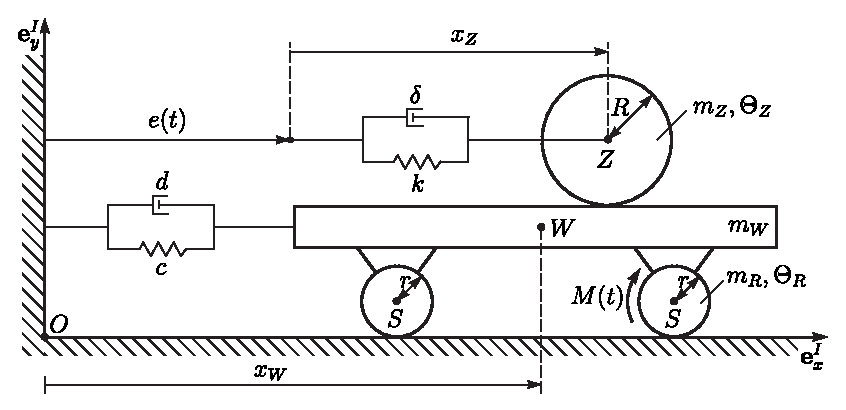
\includegraphics{graphics/Wagen.eps}
 \caption{Eine Aufgabe aus der Vorlesung TM\,III.}
 \label{wagenfig}
\end{figure}

\section{Formeln}
Vektorgrößen schreibt man in der Regel mit kleinen fetten lateinischen Buchstaben, z.B.\ $\vx$, $\vy$, $\vz$, und manchmal mit kleinen fetten griechischen Buchstaben, z.B.\ $\val$, $\vbe$, $\vga$. Schauen Sie sich die Befehle in \verb"commands.txt" an. Matrixgrößen schreibt man in der Regel mit großen fetten lateinischen Buchstaben, z.B.\ $\vA$, $\vB$, $\vC$. Nur in Einzelfällen weicht man von diesen Regeln ab um die übliche Notation der klassischen Mechanik zu respektieren. Der Spinsatz, zum Beispiel, wird in der Vorlesung Technische Mechanik als
\begin{equation}\label{spinsatz}
 \dot{\vN}_S = \vTh_S\,\vPs + \vOm\times\vTh_S\,\vOm =
 \vM_S^\mathrm{a}
\end{equation}
geschrieben. Koordinatensysteme werden geschrieben als $(O, \ve_x^I, \ve_y^I, \ve_z^I)$ und Matrizen beispielsweise als
\begin{equation}
 _K\vTh_S = \begin{pmatrix}
              A & D & E\\
              D & B & F\\
              E & F & C
            \end{pmatrix}.
\end{equation}
Formeln sind mit den Befehlen in \verb"commands.tex" zu erstellen. Nach Bedarf können eigene Befehle hinzugefügt werden.
\newpage
\section{Literatur}
Das Literaturverzeichnis ist mit Bibtex zu erstellen. Das Ausgabeprofil in TeXnicCenter beinhaltet einen entsprechenden Bibtex Aufruf. Die Vorlage \verb"literatur.bib" enthält schon einige Beispiele, z.B.\ \cite{Lein2002,Lein2003,Lein2004,Lein2005,Lein2006,Lein2007}. JabRef ist ein angenehmes und frei verfügbares Programm um \verb".bib"-Dateien zu erstellen und eine Literaturdatenbank aufzubauen. Die Quelldatei \verb"literatur.bib" ist wie alle Latex-Dateien dieser Vorlage \verb"UTF-8" kodiert. Umlaute und Sonderzeichen (z.B.\ ä, ü, ö, ß) können somit direkt verwendet werden.
